
(b) With a Langevin (Metropolis-Hastings) algorithm with proposals $Y_n$~$N(X_{n-1}+\frac{1}{2}\sigma^2g'(X_{n-1})/g(X_{n-1}),\sigma^2)$.
First we calculate analycically $g'(x)$:
\begin{align*}
\frac{dg}{dx} &= 
\begin{cases}
  \frac{d}{dx}\left(e^{-x/10}(1+\cos(x)\sin(x^3))\right) &\text{for }x>0\\
  \frac{d}{dx}\left(e^{x/10}(1+\cos(x)\sin(x^3))\right) &\text{for }x<0
\end{cases}\\
  &=\begin{cases}
  -\frac{1}{10}e^{-x/10}(1+\cos(x)\sin(x^3)) +e^{-x/10}(3x^2\cos(x)\cos(x^3)-\sin(x)\sin(x^3)) &\text{for }x>0\\
  \frac{1}{10}e^{x/10}(1+\cos(x)\sin(x^3)) +e^{x/10}(3x^2\cos(x)\cos(x^3)-\sin(x)\sin(x^3)) &\text{for }x<0\\
  \end{cases}
\end{align*}
With the closed form of $g'(x)$ calculated, we can implement the Langevin algorithm with the following code
\begin{knitrout}
\definecolor{shadecolor}{rgb}{0.969, 0.969, 0.969}\color{fgcolor}\begin{kframe}
\begin{alltt}
\hlcom{#Estimate E_pi(X+X^2) where pi=cg using Metropolis-Hasting algorithm where}
\hlcom{# g(x) = e^(-|x|/10)*(1+cos(x)sin(x^3))}
\hlcom{# with proposal N(X_(n-1)+1/2sigma^2g'(X_(n-1)),sigma^2)}

\hlstd{sigma} \hlkwb{=} \hlnum{0.1}
\hlstd{M} \hlkwb{=}\hlnum{1e5}
\hlstd{B} \hlkwb{=} \hlnum{2e4}

\hlstd{fn} \hlkwb{=} \hlkwa{function}\hlstd{(}\hlkwc{x}\hlstd{) \{x}\hlopt{+}\hlstd{x}\hlopt{^}\hlnum{2}\hlstd{\}}
\hlstd{g} \hlkwb{=} \hlkwa{function}\hlstd{(}\hlkwc{x}\hlstd{) \{}\hlkwd{exp}\hlstd{(}\hlopt{-}\hlkwd{abs}\hlstd{(x)}\hlopt{/}\hlnum{10}\hlstd{)}\hlopt{*}\hlstd{(}\hlnum{1}\hlopt{+}\hlkwd{cos}\hlstd{(x)}\hlopt{*}\hlkwd{sin}\hlstd{(x}\hlopt{^}\hlnum{3}\hlstd{))\}}
\hlstd{gp} \hlkwb{=} \hlkwa{function}\hlstd{(}\hlkwc{x}\hlstd{) \{}
  \hlkwa{if} \hlstd{(x}\hlopt{>=}\hlnum{0}\hlstd{)}
    \hlopt{-}\hlkwd{exp}\hlstd{(}\hlopt{-}\hlstd{x}\hlopt{/}\hlnum{10}\hlstd{)}\hlopt{/}\hlnum{10}\hlopt{*}\hlstd{(}\hlnum{1}\hlopt{+}\hlkwd{cos}\hlstd{(x)}\hlopt{*}\hlkwd{sin}\hlstd{(x}\hlopt{^}\hlnum{3}\hlstd{))}\hlopt{+}\hlkwd{exp}\hlstd{(}\hlopt{-}\hlstd{x}\hlopt{/}\hlnum{10}\hlstd{)}\hlopt{*}\hlstd{(}\hlnum{3}\hlopt{*}\hlstd{x}\hlopt{^}\hlnum{2}\hlopt{*}\hlkwd{cos}\hlstd{(x)}\hlopt{*}\hlkwd{cos}\hlstd{(x}\hlopt{^}\hlnum{3}\hlstd{)}\hlopt{-}\hlkwd{sin}\hlstd{(x)}\hlopt{*}\hlkwd{sin}\hlstd{(x}\hlopt{^}\hlnum{3}\hlstd{))}
  \hlkwa{else}
    \hlkwd{exp}\hlstd{(x}\hlopt{/}\hlnum{10}\hlstd{)}\hlopt{/}\hlnum{10}\hlopt{*}\hlstd{(}\hlnum{1}\hlopt{+}\hlkwd{cos}\hlstd{(x)}\hlopt{*}\hlkwd{sin}\hlstd{(x}\hlopt{^}\hlnum{3}\hlstd{))}\hlopt{+}\hlkwd{exp}\hlstd{(x}\hlopt{/}\hlnum{10}\hlstd{)}\hlopt{*}\hlstd{(}\hlnum{3}\hlopt{*}\hlstd{x}\hlopt{^}\hlnum{2}\hlopt{*}\hlkwd{cos}\hlstd{(x)}\hlopt{*}\hlkwd{cos}\hlstd{(x}\hlopt{^}\hlnum{3}\hlstd{)}\hlopt{-}\hlkwd{sin}\hlstd{(x)}\hlopt{*}\hlkwd{sin}\hlstd{(x}\hlopt{^}\hlnum{3}\hlstd{))}
\hlstd{\}}
\hlstd{qq} \hlkwb{=} \hlkwa{function}\hlstd{(}\hlkwc{x}\hlstd{,}\hlkwc{y}\hlstd{) \{}
  \hlkwd{exp}\hlstd{(}\hlopt{-}\hlstd{(y}\hlopt{-}\hlstd{x}\hlopt{-}\hlstd{sigma}\hlopt{^}\hlnum{2}\hlopt{*}\hlkwd{gp}\hlstd{(x)}\hlopt{/}\hlkwd{g}\hlstd{(x)}\hlopt{/}\hlnum{2}\hlstd{)}\hlopt{^}\hlnum{2}\hlopt{/}\hlstd{sigma}\hlopt{^}\hlnum{2}\hlopt{/}\hlnum{2}\hlstd{)}
\hlstd{\}}

\hlcom{#initialization}
\hlstd{fnlist} \hlkwb{=} \hlkwd{numeric}\hlstd{(M}\hlopt{+}\hlstd{B)}
\hlstd{xlist} \hlkwb{=} \hlkwd{numeric}\hlstd{(M}\hlopt{+}\hlstd{B)}
\hlstd{x} \hlkwb{=} \hlkwd{rnorm}\hlstd{(}\hlnum{1}\hlstd{,}\hlnum{0}\hlstd{,sigma)}
\hlstd{acc} \hlkwb{=} \hlnum{0}

\hlkwa{for} \hlstd{(i} \hlkwa{in} \hlnum{1}\hlopt{:}\hlstd{(M}\hlopt{+}\hlstd{B)) \{}

  \hlstd{m} \hlkwb{=} \hlnum{1}\hlopt{/}\hlnum{2}\hlopt{*}\hlstd{sigma}\hlopt{^}\hlnum{2}\hlopt{*}\hlkwd{gp}\hlstd{(x)}\hlopt{/}\hlkwd{g}\hlstd{(x)}
  \hlstd{y} \hlkwb{=} \hlkwd{rnorm}\hlstd{(}\hlnum{1}\hlstd{,x}\hlopt{+}\hlstd{m,sigma)}

  \hlkwa{if} \hlstd{(}\hlkwd{runif}\hlstd{(}\hlnum{1}\hlstd{)}\hlopt{<=}\hlkwd{g}\hlstd{(y)}\hlopt{*}\hlkwd{qq}\hlstd{(y,x)}\hlopt{/}\hlkwd{g}\hlstd{(x)}\hlopt{/}\hlkwd{qq}\hlstd{(x,y)) \{}
    \hlkwa{if} \hlstd{(i}\hlopt{>}\hlstd{B)}
      \hlstd{acc}\hlkwb{=}\hlstd{acc}\hlopt{+}\hlnum{1}
    \hlstd{x} \hlkwb{=} \hlstd{y}
  \hlstd{\}}
  \hlstd{xlist[i]} \hlkwb{=} \hlstd{x}
  \hlstd{fnlist[i]} \hlkwb{=} \hlkwd{fn}\hlstd{(x)}
\hlstd{\}}

\hlstd{funcmean} \hlkwb{=} \hlkwd{mean}\hlstd{(fnlist[(B}\hlopt{+}\hlnum{1}\hlstd{)}\hlopt{:}\hlstd{(M}\hlopt{+}\hlstd{B)])}
\hlstd{funciidse} \hlkwb{=} \hlkwd{sd}\hlstd{(fnlist[(B}\hlopt{+}\hlnum{1}\hlstd{)}\hlopt{:}\hlstd{(M}\hlopt{+}\hlstd{B)])}\hlopt{/}\hlkwd{sqrt}\hlstd{(M)}
\hlstd{acf_k} \hlkwb{=} \hlkwd{acf}\hlstd{(fnlist[(B}\hlopt{+}\hlnum{1}\hlstd{)}\hlopt{:}\hlstd{(M}\hlopt{+}\hlstd{B)],}\hlkwc{lag.max} \hlstd{=} \hlnum{1000}\hlstd{,}\hlkwc{plot} \hlstd{=} \hlnum{FALSE}\hlstd{)}\hlopt{$}\hlstd{acf}
\hlstd{varfact} \hlkwb{=} \hlnum{2}\hlopt{*}\hlkwd{sum}\hlstd{(acf_k)}\hlopt{-}\hlnum{1}
\hlstd{funcse} \hlkwb{=} \hlstd{funciidse}\hlopt{*}\hlkwd{sqrt}\hlstd{(varfact)}
\hlstd{accrate} \hlkwb{=} \hlstd{acc}\hlopt{/}\hlstd{M}

\hlkwd{cat}\hlstd{(}\hlstr{'B = '}\hlstd{,B,}\hlstr{', M = '}\hlstd{,M,}\hlstr{'\textbackslash{}n'}\hlstd{)}
\hlkwd{cat}\hlstd{(}\hlstr{'Number of samples accepted = '}\hlstd{,acc,}\hlstr{', acceptance rate = '}\hlstd{,accrate,}\hlstr{'\textbackslash{}n'}\hlstd{)}
\hlkwd{cat}\hlstd{(}\hlstr{'Estimate = '}\hlstd{,funcmean,}\hlstr{'\textbackslash{}n'}\hlstd{)}
\hlkwd{cat}\hlstd{(}\hlstr{'i.i.d. standard error = '}\hlstd{,funciidse,}\hlstr{'\textbackslash{}n'}\hlstd{)}
\hlkwd{cat}\hlstd{(}\hlstr{'varfact = '}\hlstd{,varfact,}\hlstr{'\textbackslash{}n'}\hlstd{)}
\hlkwd{cat}\hlstd{(}\hlstr{'Standard error = '}\hlstd{,funcse,}\hlstr{'\textbackslash{}n'}\hlstd{)}
\end{alltt}
\end{kframe}
\end{knitrout}
Output of several runs:
\begin{knitrout}
\definecolor{shadecolor}{rgb}{0.969, 0.969, 0.969}\color{fgcolor}\begin{kframe}
\begin{verbatim}
## B =  20000 , M =  1e+05 
## Number of samples accepted =  72892 , acceptance rate =  0.72892 
## Estimate =  16.37651 
## i.i.d. standard error =  0.07014971 
## varfact =  1875.972 
## Standard error =  3.038359
## B =  20000 , M =  1e+05 
## Number of samples accepted =  66806 , acceptance rate =  0.66806 
## Estimate =  51.28206 
## i.i.d. standard error =  0.2649013 
## varfact =  1958.284 
## Standard error =  11.72255
## B =  20000 , M =  1e+05 
## Number of samples accepted =  55956 , acceptance rate =  0.55956 
## Estimate =  23.24639 
## i.i.d. standard error =  0.06920837 
## varfact =  1798.478 
## Standard error =  2.935021
## B =  20000 , M =  1e+05 
## Number of samples accepted =  64279 , acceptance rate =  0.64279 
## Estimate =  18.73548 
## i.i.d. standard error =  0.06656209 
## varfact =  1821.751 
## Standard error =  2.841001
## B =  20000 , M =  1e+05 
## Number of samples accepted =  76744 , acceptance rate =  0.76744 
## Estimate =  8.867096 
## i.i.d. standard error =  0.03519465 
## varfact =  1715.128 
## Standard error =  1.457555
\end{verbatim}
\end{kframe}
\end{knitrout}
The tabulated result is as follows:\\
\begin{center}
\begin{knitrout}
\definecolor{shadecolor}{rgb}{0.969, 0.969, 0.969}\color{fgcolor}
\begin{tabular}{r|r|r|r|r}
\hline
estimation & acc\_rate & seiid & varfact\_r & standard\_error\\
\hline
16.376511 & 0.72892 & 0.0701497 & 1875.972 & 3.038359\\
\hline
51.282063 & 0.66806 & 0.2649013 & 1958.284 & 11.722547\\
\hline
23.246395 & 0.55956 & 0.0692084 & 1798.478 & 2.935021\\
\hline
18.735479 & 0.64279 & 0.0665621 & 1821.751 & 2.841001\\
\hline
8.867096 & 0.76744 & 0.0351946 & 1715.128 & 1.457555\\
\hline
\end{tabular}


\end{knitrout}
\end{center}
We notice that the varfact values are quite small, indicating that the samples are not strongly correlated. To verify the effectiveness of the sampler, here we plot the value of $x$ after the burn-in stage
\begin{figure}[H]
  \centering
\begin{knitrout}
\definecolor{shadecolor}{rgb}{0.969, 0.969, 0.969}\color{fgcolor}\begin{kframe}
\begin{alltt}
\hlstd{xlist8b} \hlkwb{=} \hlstd{xlist}
\hlkwd{plot}\hlstd{(xlist8b[(B}\hlopt{+}\hlnum{1}\hlstd{)}\hlopt{:}\hlstd{(B}\hlopt{+}\hlstd{M)],}\hlkwc{type}\hlstd{=}\hlstr{'l'}\hlstd{)}
\end{alltt}
\end{kframe}
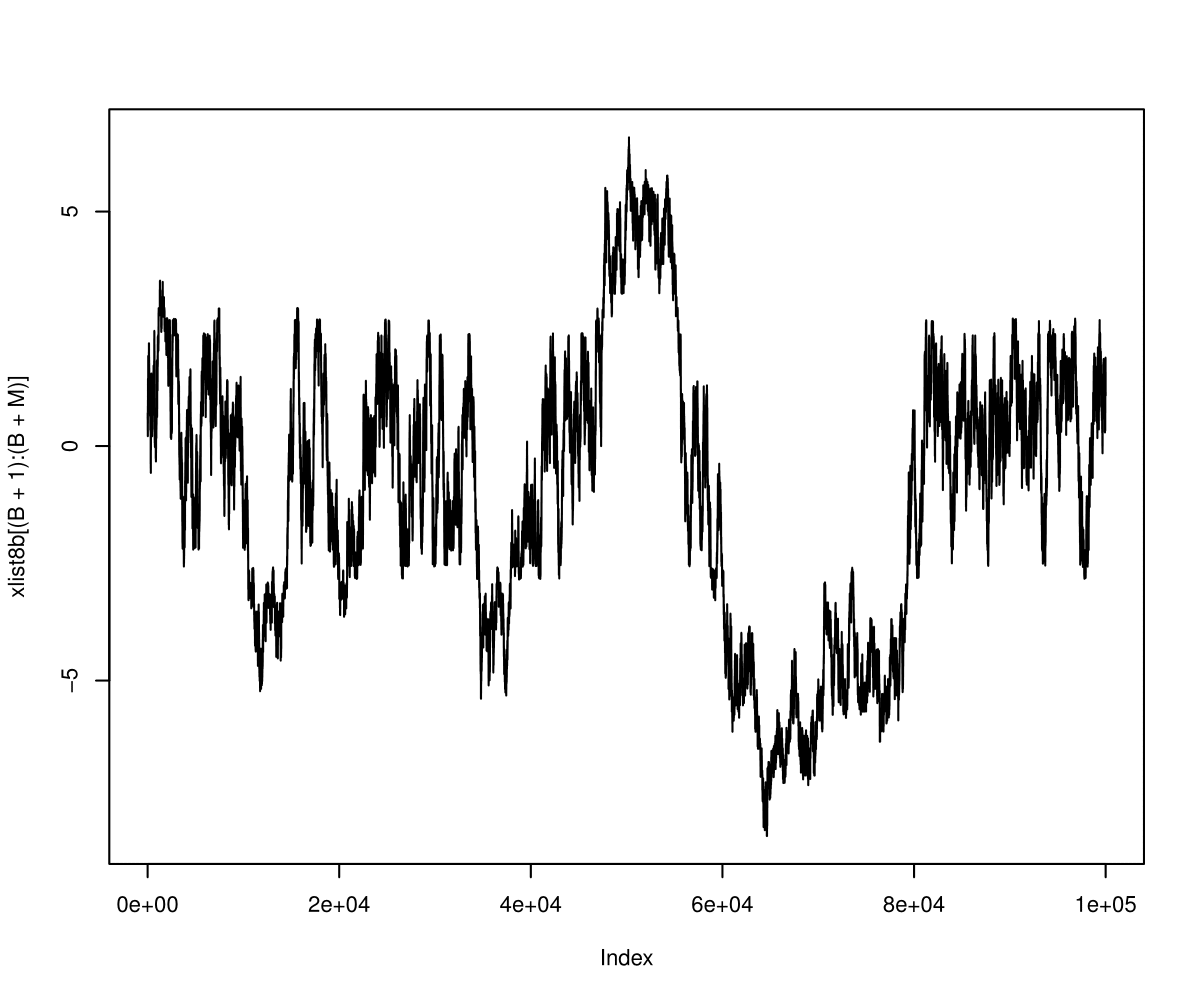
\includegraphics[width=\maxwidth]{figure/p8bplot-1} 

\end{knitrout}
		\caption{$x$ values of Langevin algorithm after burning-in}
\end{figure}

Notice that the estimation is by no means consistent, and the varfact values are huge, making the standar error large too.\\
\\
(c) Compare the two algorithms and discuss which one is "better".\\
In this case, the random-walk Metropolis algorithm clearly outperforms the Langevin algorithm as it produces more reasonable estimates to the integral. The Langevin algorithm is designed to work well for well behaved functions. In particular, if the function $g'(x)/g(x)$ is smooth, then the Langevin algorithm is going to outperform RWM algorithm. However, if we plot $g'(x)/g(x)$, we notice that it varies significantly even on a log-scaled plot
\begin{figure}[H]
  \centering
\begin{knitrout}
\definecolor{shadecolor}{rgb}{0.969, 0.969, 0.969}\color{fgcolor}\begin{kframe}
\begin{alltt}
\hlstd{xline} \hlkwb{=} \hlkwd{seq}\hlstd{(}\hlopt{-}\hlnum{10}\hlstd{,}\hlnum{10}\hlstd{,}\hlnum{0.01}\hlstd{)}
\hlkwd{plot}\hlstd{(}\hlkwd{log}\hlstd{(}\hlkwd{gp}\hlstd{(xline)}\hlopt{/}\hlkwd{g}\hlstd{(xline)),}\hlkwc{type}\hlstd{=}\hlstr{'l'}\hlstd{)}
\end{alltt}


{\ttfamily\noindent\color{warningcolor}{\#\# Warning in if (x >= 0) -exp(-x/10)/10 * (1 + cos(x) * sin(x\textasciicircum{}3)) + exp(-x/10) * : the condition has length > 1 and only the first element will be used}}

{\ttfamily\noindent\color{warningcolor}{\#\# Warning in log(gp(xline)/g(xline)): NaNs produced}}\end{kframe}
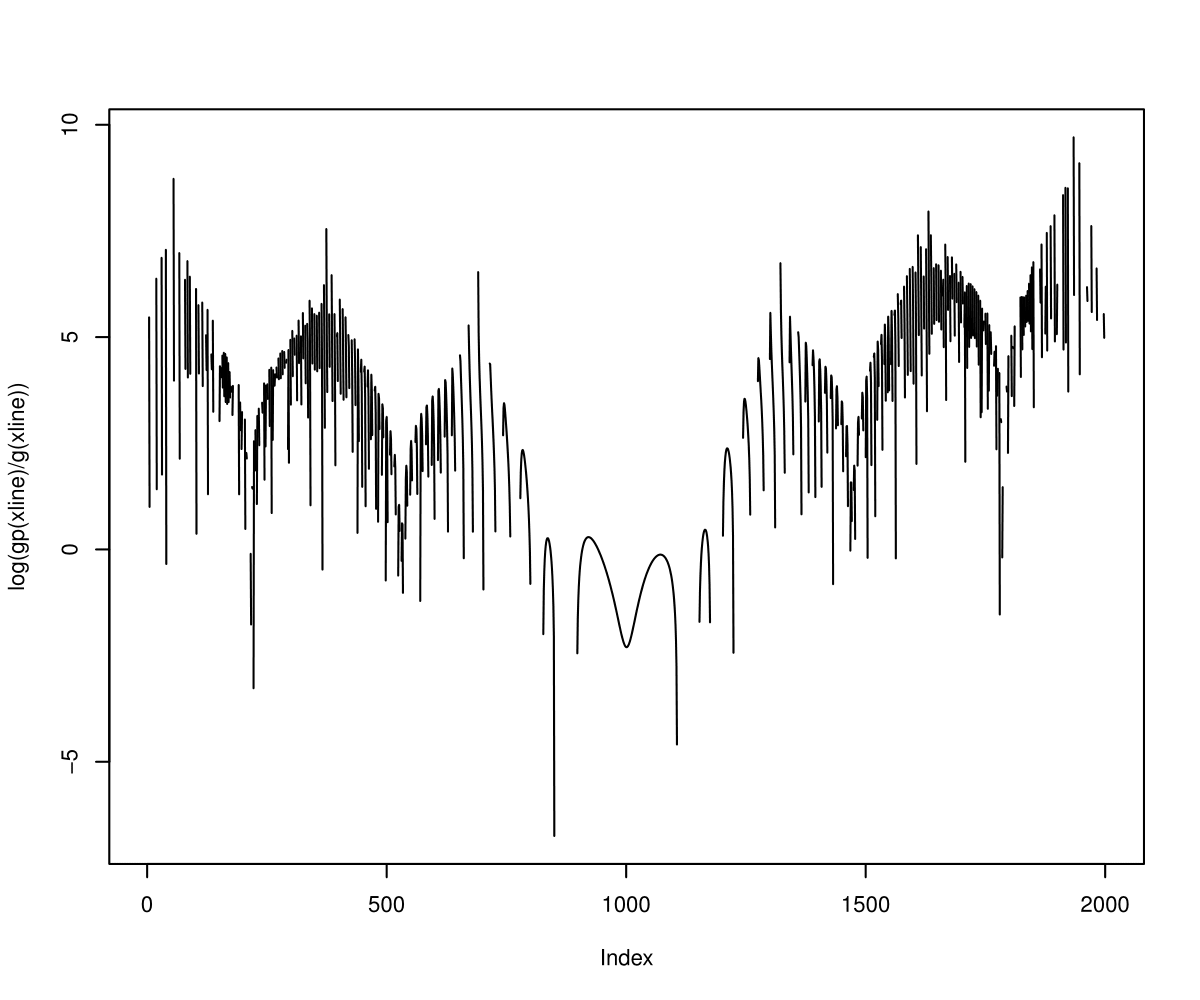
\includegraphics[width=\maxwidth]{figure/p8cplot-1} 

\end{knitrout}
\end{figure}
Since to the function $g'(x)/g(x)$ is unstable, a discrete approximation of this function will fail. As a result, the RWM algorithm outperforms the Langevin algorithm significantly.
